\documentclass{article}
\usepackage[utf8]{inputenc}
\usepackage{amsmath}
\usepackage{amssymb}
\usepackage{mathtools}
\usepackage{tikz}
\usetikzlibrary{arrows,shapes,positioning}

\usepackage{dirtytalk}

\title{The Basics of Option Pricing}
\author{Gerardo Durán Martín}

\newtheorem{theorem}{Theorem}[section]

\begin{document}
\maketitle


\section{Introduction}
Broadly speaking, financial instruments can be grouped into two distinct categories: \textit{underlying}s and \textit{derivatives}. The former refers to stocks, bonds, commodities, foreign exchange currencies, etc; while the latter refers to any \say{financial instrument whose value depends on (or derives from) the value of other, more basic, underlying variables} (Hull 2015).\\

A financial institution might be interested in selling these derivatives as a service and charge a fee for it. The question then arises, how much should the financial institution charge for these products? As a first attempt to \textit{price} any of these derivatives, one could charge the expected value of the derivative in the future, discounted at some rate $r$. Simply put, assuming we can sell many units of a given product, by \textbf{Kolmogorov's Strong Law of Large Numbers (LLN)}, we would expect, in the long run, to break even:

\begin{theorem}
    Let $\{X_n\}_{n\geq 1}$ be a collection of i.i.d. random variables with mean $\mu$. Denote $S_n = \frac{1}{n}\sum_{i=1}^n X_n$. Then, with probability one,
    \begin{equation}
        S_n \xrightarrow[n \rightarrow \infty]{}\mu
    \end{equation}
\end{theorem}


%%% TODO: write about the failure of this approach by pricing a forward that could lead to arbitrage and a loss for the financial institution
Feasible as it may seem, as pointed out by Baxter(2003), this approach could lead to disaster for the financial institution.


\section{One-Step Binomial Models}
In order to generalize an arbitrage-free approach to price any derivative, we would like to construct a model that truly reflects the market (unlike the LLN approach). In its simplest form, this market should consist of a cash bond and a stock. We will assume, that the market moves in discrete units of time.\\

\textbf{The Stock}\\
Between any two units of time (e.g. from $t=0$ to $t=1$), the stock can either go up with probability $p$, or down with probability $1-p$; it will have an initial value $S_0$ and, with any of these movements, the stock is multiplied by an up factor $u$, or a down factor $d$, depending on where it moves to. Evidently, $0 < d < 1 < u$. Finally, we will assume that unlimited amounts of the stock can be bought at any time and there is no cost incurred.

\begin{center}
\begin{tikzpicture}
    \draw[->] (0,0) node[left]{$S_0$} --(2, 0.5) node[pos=0.5, sloped, above] {$p$};
    \node[text, right] at (2, 0.5) {$S_0u$};

    \draw[->] (0,0) --(2, -0.5) node[pos=0.5, sloped, below] {$1-p$};
    \node[text, right] at (2, -0.5) {$S_0d$};
\end{tikzpicture}
\end{center}

\textbf{The Bond}\\
The bank account represents the time value of money. We will assume a constant, risk-free, continuously compounding interest rate $r$. For $\$B_0$ invested at $t=0$, said rate guarantees, at the end of $T$ periods, $B_0 e^{rT}$. Also, we will assume that we can lend or borrow at the same interest rate $r$.\\

\textbf{The Derivative}\\
This model carries within the possibility of a market that depends on the price of the stock. That is, there could be a payoff $f$ with price $f_0$ that derives its future value from the direction the stock took. Either $f_u$ if it went up, or $f_d$ if it went down.

\subsection{Pricing}
We can now ask whether we can construct a portfolio such that replicates $f$ from a suitable strategy, thus paying the promised amount. What we are looking for is to guarantee the value of the derivative at the moment of settlement, thus hedging the risk away.\\

Consider the portfolio $(\phi, \psi)$, where $\phi$ denotes the number of shares for stock $S$ in the portfolio and $\psi$ denotes the amount in the bank. At $t=0$, this portfolio is worth

\begin{equation*}
    \phi S_0 + \psi B_0
\end{equation*}

At $t=\delta t$, this portfolio will be worth one of two possible values:

\begin{align*}
    \phi S_0u + \psi B_0e^{r \delta t}\\
    \phi S_0d + \psi B_0e^{r \delta t}
\end{align*}

With this in mind, we now turn to answer our question. In order to hedge the risk, we would like to find values for $(\phi, \psi)$ in order to replicate the payoff:

\begin{align*}
    \phi S_0u + \psi B_0e^{r \delta t} = f_u\\
    \phi S_0d + \psi B_0e^{r \delta t} = f_d
\end{align*}

We can now solve for $\phi$ and $\psi$:

\begin{equation*}
    \phi S_0(u - d) = f_u - f_d\\
\end{equation*}

\begin{equation} \label{eq:phi}
    \phi = \frac{f_u - f_d}{S_0(u-d)}
\end{equation}

\begin{align*}
    \psi &= e^{-r\delta t} [f_u - \phi u]\\
         &= e^{-r\delta t} \left[f_u - \frac{f_u - f_d}{S_0(u - d)} S_0u\right]\\
         &= e^{-r\delta t} \frac{uf_d - df_u}{u -d}
\end{align*}

Thus, buying the portfolio $(\phi, \psi)$ guaranteed the payoff at $t=\delta_t$. Denote $\mathcal{V}$ the value of the portfolio at $t=0$. The value of $\mathcal{V}$ is:

\begin{align*}
    \mathcal{V} &= \phi S_0 + \psi\\
                &= \left[\frac{f_u - f_d}{S_0(u - d)}S_0\right] + \left[e^{-r\delta_t}\right]\\
                &= e^{-r\delta_t}\left[\frac{e^{r\delta_t}(f_u - f_d + uf_d - df_u)}{u - d}\right]\\
                &= e^{-r\delta_t}\left[\frac{e^{r\delta_t}f_u - df_u}{u-d} + \frac{uf_d - e^{r\delta_t}f_d}{u-d}\right]
\end{align*}

\begin{equation} \label{eq:v_price_complete}
    \therefore \mathcal{V} = e^{-r\delta_t}\left[f_u \frac{e^{r\delta_t} - d}{u - d} + f_d \frac{u - e^{r\delta_t}}{u-d}\right]
\end{equation}

$\mathcal{V}$ is the arbitrage-free price for this derivative. Consider any other price $\mathcal{P} < \mathcal{V}$. Buying the portfolio $\mathcal{P}$ and selling $\mathcal{V}$ at $t=0$ guarantees, at $t=\delta_t$, enough money to settle and earn $\mathcal{V}-\mathcal{P}$ risk-free. The same argument can be done for a value $\mathcal{P} > \mathcal{V}$.\\

What, then, would have happened, had we decided to replicate this payoff using only the bank account and the probabilities $p$ and $1-p$? Accordingly, we would've priced the derivative at the present value of the expected payoff under the $\mathbb{P}$ measure. Denote $\hat{\mathcal{V}}$ this alternate value, then:

\begin{equation}
    \hat{\mathcal{V}} = \exp(-r\delta_t)\mathbb{E}[f] = \exp(-r\delta_t)[f_u \cdot p + f_d \cdot (1- p) ]
\end{equation}\\


Pricing $\hat{\mathcal{V}}$ for $f$ does not guarantee $\hat{\mathcal{V}} = \mathcal{V}$, which could lead to arbitrage otherwise. Assuming $\hat{\mathcal{V}} \neq \mathcal{V}$, the expected payoff of $f$ would not be $\hat{\mathcal{V}}$, investors would be inclined to make a profit, thereby breaking the assumption that every position taken on the derivative is independent of one another; we cannot expect to break even in the long run.


\subsection{The Q Measure}
Coming back to our arbitrage-free price 

\begin{equation*}
    \mathcal{V} = e^{-r\delta_t}\left[f_u \frac{e^{r\delta_t} - d}{u - d} + f_d \frac{u - e^{r\delta_t}}{u-d}\right]
\end{equation*}

Denote
\begin{equation}
    q:= \frac{\exp{r\delta_t} - d}{u - d} \Longrightarrow 1-q = \frac{u - \exp{(r\delta_t)}}{u-d}
\end{equation}\\

We can argue that $d < \exp{(r\delta_t)} < u$ implies no arbitrage. To see why, 
\begin{enumerate}
\item Suppose $\exp{(r\delta_t)} < d < u$.\\
    At t=0 we can borrow $\$S_0$ and buy the stock. At $t=1$, we collect either $S_0u$ or $S_0d$, thereby making a risk-free profit of $S_0(u - \exp{(r\delta_t)})$ or $S_0(d - \exp{(r\delta_t)})$

\item Suppose $d < u < \exp{(r\delta_t)}$\\
    At $t=0$, lend $\$S_0$ and short the stock. At $t=1$, collect $\S_0\exp{(r\delta_t)}$ and buy the stock at either $S_0u$ or $S_0d$. Again, this guarantees a risk-free profit of either $S_0(\exp{(r\delta_t)} - u)$ or $S_0(\exp{(r\delta_t)} - d)$
\end{enumerate}

Being $d < \exp{(r\delta_t)} < u$ implies $0 < q < 1$. We can rewrite \ref{eq:v_price_complete} as

\begin{equation} \label{eq:v_price}
    \mathcal{V} = \exp{(-r\delta_t)}[S_0u\cdot q + S_0d \cdot (1-q)]
\end{equation}

$\mathcal V$ is the expectation under a measure probability $\mathbb Q$; it not the expected value of the derivative, but a change in the measure of the tree such that guarantees no arbitrage.

\section{$n$-period Binomial Tree Model}
In order to generalize our model to $n$ periods we only need to consider each node as the root of another binomial tree. Consequently, we get a tree with $n$ periods and $2^n$ nodes at $t=n$.

\begin{center}
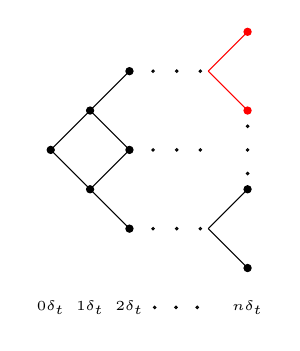
\begin{tikzpicture}
    % First Node
    \draw[-] (0,0) -- (0.5, 0.5);
    \draw[-] (0,0) -- (0.5, -0.5);
    \draw[black, fill=black](0.5,-0.5) circle (.3ex);
    \draw[black, fill=black](0.5,0.5) circle (.3ex); 
    \draw[black, fill=black](0,0) circle (.3ex);

    % 1) up node
    \draw[-](0.5, 0.5) -- (1, 1);
    \draw[-](0.5, 0.5) -- (1, 0);
    \draw[fill=black] (1,1) circle (.3ex);
    \draw[fill=black] (1,0) circle (.3ex);
    % 1) down node 
    \draw[-](0.5, -0.5) -- (1, 0);
    \draw[-](0.5, -0.5) -- (1, -1);
    \draw[fill=black] (1,-1) circle (.3ex);
    
    % Connection points
    \draw[black](1.3, 1) circle (.1ex);
    \draw[black](1.6, 1) circle (.1ex);
    \draw[black](1.9, 1) circle (.1ex);

    \draw[black](1.3, 0) circle (.1ex);
    \draw[black](1.6, 0) circle (.1ex);
    \draw[black](1.9, 0) circle (.1ex);


    \draw[black](1.3, -1) circle (.1ex);
    \draw[black](1.6, -1) circle (.1ex);
    \draw[black](1.9, -1) circle (.1ex);
    
    \draw[black](2.5, 0.3) circle (.1ex);
    \draw[black](2.5, 0) circle (.1ex);
    \draw[black](2.5, -0.3) circle (.1ex);

    % 2.1) up node
    \draw[-, red](2, 1) -- (2.5, 1.5);
    \draw[-, red](2, 1) -- (2.5, 0.5);
    \draw[red, fill=red] (2.5, 1.5) circle (.3ex);
    \draw[red, fill=red] (2.5,0.5) circle (.3ex);
    % 2.2) down node 
    \draw[-](2, -1) -- (2.5, -0.5);
    \draw[-](2, -1) -- (2.5, -1.5);
    \draw[fill=black] (2.5,-0.5) circle (.3ex);
    \draw[fill=black] (2.5,-1.5) circle (.3ex);

    \node[font=\fontsize{4}{4}] at (0, -2) {$0\delta_t$};
    \node[font=\fontsize{4}{4}] at (0.5, -2) {$1\delta_t$};
    \node[font=\fontsize{4}{4}] at (1, -2) {$2\delta_t$};
    \draw (1.32, -2) circle (.1ex);
    \draw (1.59, -2) circle (.1ex);
    \draw (1.86, -2) circle (.1ex);
    \node[font=\fontsize{4}{4}] at (2.5, -2) {$n\delta_t$};
\end{tikzpicture}\\
\caption{Fig: the $n$-period model}
\end{center}

To motivate this generalized model, we will now present an example of a $3$-period binomial model.
% Find another name for this example...
\subsection{An Example}
Suppose that at $t=0$ we have a stock $S_0$ that can go up up by a factor of $1.20$, or down by a factor of $0.80$. Assume further that the $\mathbb{P}$ measure probability for an up move is $\frac{3}{4}$, finally, suppose $r=0$. Being consistent with the notation used, $u=1.20$, $d=0.80$, $p = \frac{3}{4}$ and $ 1 - p = \frac{1}{4}$. We want to price a call option on $S_0$ with strike price $k=100$.Denote this claim, at $t=4$, $f$, and $S_n$ as the value of $S$ at maturity. We can represent this claim as:

\begin{equation}
    f = [S_n - k]^+
\end{equation}

Since the stock can either move up or down with known factors $u$ and $d$ respectively, we know all the values the stock can take up to $t=3$. For example, from $t=0$ to $t=1$, the stock can either move to $100 \cdot 1.20$, or down to $100 \cdot 0.80$.

\begin{center}
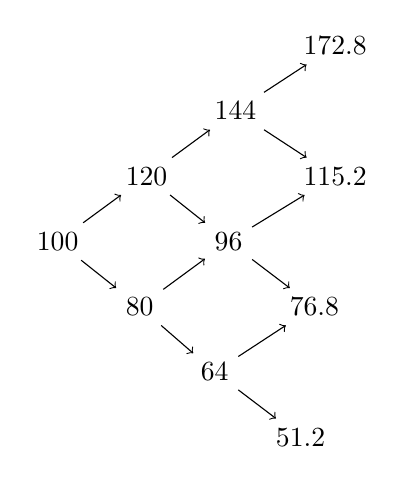
\begin{tikzpicture}
    \node (s) at (0,0) {100};

    \node[above right = 0.5cm of s] (su) {120}; \draw[->] (s) -- (su);
    \node[below right = 0.5cm of s] (sd) {80};  \draw[->] (s) -- (sd);

    \node[above right = 0.5cm of su] (suu) {144}; \draw[->] (su) -- (suu);
    \node[below right = 0.5cm of su] (sud) { 96}; \draw[->] (su) -- (sud); \draw[->] (sd) -- (sud);
    \node[below right = 0.5cm of sd] (sdd) { 64}; \draw[->] (sd) -- (sdd);

    \node[above right = 0.5cm of suu] (suuu) {172.8}; \draw[->] (suu) -- (suuu);
    \node[below right = 0.5cm of suu] (suud) {115.2}; \draw[->] (suu) -- (suud); \draw[->] (sud) -- (suud);
    \node[below right = 0.5cm of sud] (sudd) { 76.8}; \draw[->] (sud) -- (sudd); \draw[->] (sdd) -- (sudd);
    \node[below right = 0.5cm of sdd] (sddd) { 51.2}; \draw[->] (sdd) -- (sddd);
\end{tikzpicture}\\
\caption{Fig: The Stock Process}
\end{center}

Given $f$ and the stock-tree process we can compute, for example, the amount to be paid if the stock moves up at every step. Under this scenario, $S_3 = 172.8$. Then $f(S_3) = [172.8 - 110]^+ = 62.80$, which means that the buyer of the option would receive $\$62.80$. Computing the claim at every last node yields a set of claims at maturity.\\

With the set of claims at maturity, we proceed to find the value of the option at every other node in the tree solving iteratively from $t=2$ to $t=0$.\\

For example, the upper node at $t=2$ is computed by taking the discounted expectation under the $\mathbb{Q}$ measure as shown in \ref{eq:v_price}. Were the stock to climb up two times then, the payoff at $t=3$ can either be 62.8 or 5.2. Denote $f^{uu}_2$ the value the derivative at $t=2$ for the upper node, its value is then

\begin{equation*}
    f^{uu}_2 = \exp(-0)[62.8q + 5.2(1-q)] = 34; \  q = \frac{0 - 0.80}{1.20 - 0.80}
\end{equation*}\\

\begin{center}
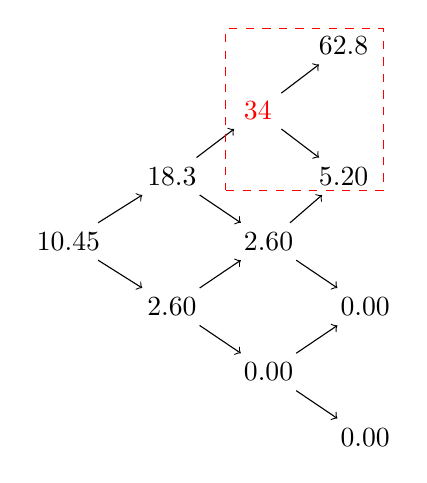
\begin{tikzpicture}
    \node (s) at (0,0) {10.45};

    \node[above right = 0.5cm of s] (su) {18.3}; \draw[->] (s) -- (su);
    \node[below right = 0.5cm of s] (sd) {2.60};  \draw[->] (s) -- (sd);

    \node[red, above right = 0.5cm of su] (suu) {34}; \draw[->] (su) -- (suu);
    \node[below right = 0.5cm of su] (sud) {2.60}; \draw[->] (su) -- (sud); \draw[->] (sd) -- (sud);
    \node[below right = 0.5cm of sd] (sdd) {0.00}; \draw[->] (sd) -- (sdd);

    \node[above right = 0.5cm of suu] (suuu) {62.8}; \draw[->] (suu) -- (suuu);
    \node[below right = 0.5cm of suu] (suud) {5.20}; \draw[->] (suu) -- (suud); \draw[->] (sud) -- (suud);
    \node[below right = 0.5cm of sud] (sudd) {0.00}; \draw[->] (sud) -- (sudd); \draw[->] (sdd) -- (sudd);
    \node[below right = 0.5cm of sdd] (sddd) {0.00}; \draw[->] (sdd) -- (sddd);

    \draw[red, dashed] (2,0.65) -- (4,0.65) -- (4, 2.7) -- (2, 2.7) -- (2, 0.65);
    \end{tikzpicture}\\
    \caption{Fig: The claim-tree} 
\end{center}

Loosely speaking, every node in the claim-tree represents the value of the option at every step. Evidently, at $t=3$, the value of the option can only be its current value since there is nowhere to move elsewhere in the tree. At $t=0$ we have the risk-free value for the option that guarantees no arbitrage.\\

To see why this is true, suppose we were to sell this option at \$10.45. For the sake of the argument, suppose the stock moves up two times and down at the last time-tick. If 10.45 is truly the arbitrage-free price option, we should be able to replicate the movement of the stock at each time interval and arrive at the payoff without incurring any other cost.\\

According to equation \ref{eq:phi}, at $t=0$ we would need to buy 0.3925 units of $S$ and borrow 28.8 to cover the expenses; if the price goes up at $t=1$, aroung 0.65 units of the stock are required, which would lead to a purchase of 0.26 extra units of the stock, thus incrementing the amount borrowed to 60.2. At $t=2$, 1 unit of $S$ is required, increasing the amount borrowed to 110. Finally, at $t=3$, the stock takes a down move and \$5.2 is the amount owed to the option buyer. \\

The final value in the position of the stock is $S_0 u ^ 2 d \cdot \phi = 115.20$, minus the \$110 owed, brings the total value of the portfolio to \$5.20, exacltly the amount required to fulfill the obligation.

\newpage
\begin{thebibliography}{1}

  \bibitem{isci} David G. Luenberger {\em Investment Science}  1998.
  \bibitem{bax} Martin Baxter, Andrew Rennie {\em Financial Calculus: An Introduction to Derivative Pricing} 2003.
  \bibitem{jaksa} Jakša Cvitanić, Fernando Zapatero {\em Introduction to the Economics and Mathematics of Financial Markets} 2004.
  \bibitem{hull} Hull, John. {\em Futures, and Other Derivatives} Upper Saddle River, NJ: Pearson/Prentice Hall, 2015. Print.

\end{thebibliography}
\end{document}
